\documentclass[tikz, border=10pt]{standalone}
\usepackage{pgfplots}
\usepackage{amsmath}
\usetikzlibrary{backgrounds}
\pgfplotsset{compat=1.18}

\begin{document}
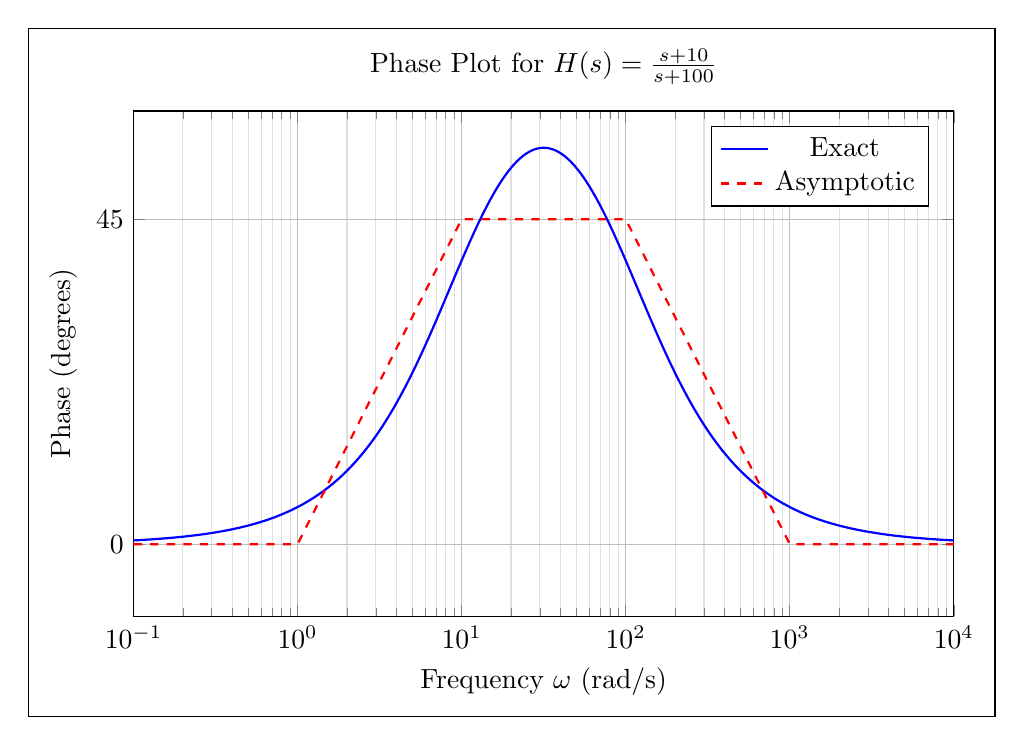
\begin{tikzpicture}[show background rectangle]
    \begin{semilogxaxis}[
        width=12cm, height=8cm,
        title={Phase Plot for $H(s) = \frac{s+10}{s+100}$},
        xlabel={Frequency $\omega$ (rad/s)},
        ylabel={Phase (degrees)},
        grid=both,
        xmin=0.1, xmax=10000,
        ymin=-10, ymax=60,
        minor grid style={gray!25},
        major grid style={gray!50},
        legend pos=north east,
        ytick={0, 45},
    ]

    % Exact Phase: atan(x/10) - atan(x/100)
    \addplot[blue, thick, domain=0.1:10000, samples=300] {atan(x/10) - atan(x/100)};
    \addlegendentry{Exact}

    % Asymptotic Phase
    % Zero at 10: 0 until 1, +45/dec to 100 (diff +90)
    % Pole at 100: 0 until 10, -45/dec to 1000 (diff -90)
    % Sum:
    % <1: 0
    % 1-10: +45/dec (ends at 45)
    % 10-100: +45-45=0/dec (flat at 45)
    % 100-1000: 0-45=-45/dec (ends at 0)
    % >1000: 0
    \addplot[red, dashed, thick] coordinates {
        (0.1, 0) (1, 0) (10, 45) (100, 45) (1000, 0) (10000, 0)
    };
    \addlegendentry{Asymptotic}
    
    \end{semilogxaxis}
\end{tikzpicture}
\end{document}
